
In this chapter, a comprehensive overview of the Bipolar Disorder Corpus is firstly provided. The literature is then given on the automatic recognition systems of bipolar disorder and AVEC2018 challenge that builds the platform for these competing systems. Some depression detection systems using multimodal data are reviewed as they share many similarities as the BD recognition system.



\section{Bipolar Disorder Corpus}
\label{sec:bp-corpus}

Bipolar disorder (BD) is a major public health problem, with estimates of lifetime prevalence in the general population of the United States at 3.9 percent, with a range from 1.5 to 6.0 percent \cite{world2017, hilty2006}. BD patients tend to have higher probability of suicide, in which approximately 25 percent attempting it and 11 percent completing it \cite{prien1990}. For medical care in BD, two challenges remain, namely access to treatment and treatment resistance \cite{bauer2017}. In spite of the recent advance in the automatic recognition of human behaviours or depression severity, a dedicated BD corpus is required to find biological markers or predictors of treatment response and to reduce treatment resistance. 

The Turkish Audio-Visual Bipolar Disorder (BD) Corpus is a new dataset for the affective computing and psychiatric communities \cite{cciftcci2018}. The corpus is also expected to provide an insight for the personalized treatment of BD patients \cite{cciftcci2018}. The corpus is annotated for BD states as well as the Young Mania Rating Scale (YMRS) by psychiatrists following DSM-5's inclusion criteria \cite{american2013}. More specifically, the YMRS scores are obtained at session level such that each score corresponds to one patient on one of the test days: $0^{th}$ day, $3^{rd}$ day, $7^{th}$ day, $14^{th}$ day, $28^{th}$ day, $90^{th}$ day. The data format in the corpus is a set of audio-visual recordings of structured interviews performed by 46 Turkish speaking objects (49 healthy controls). During the interviews, participants were asked to complete seven tasks as shown in Table \ref{tab:question}, and the two emotion-eliciting pictures used are displayed as Figure \ref{fig:drawing}.

\begin{table}[ht]
    \centering
    \caption{List of questions in the structured interviews of BD corpus}
    \begin{tabular}{l|l|l}
        \Xhline{2\arrayrulewidth}
        index & required task & topic \\
        \hline
        1 & Describe why you come here & negative task \\
        2 & Depict Van Gogh's \textit{Depression} & negative task \\
        3 & Describe the worst memory & negative task \\
        \hline
        4 & Count 1 - 30 & neutral task \\
        5 & Count 1 - 30 again (usually faster) & neutral task \\
        \hline
        6 & Depict Dengel's \textit{Home Sweet Home} & positive task \\
        7 & Describe the best memory & positive task \\
        \Xhline{2\arrayrulewidth}
    \end{tabular}
    \label{tab:question}
\end{table}

\begin{figure}[ht]
    \centering
    \begin{minipage}[c]{0.30\textwidth}
    \centering
    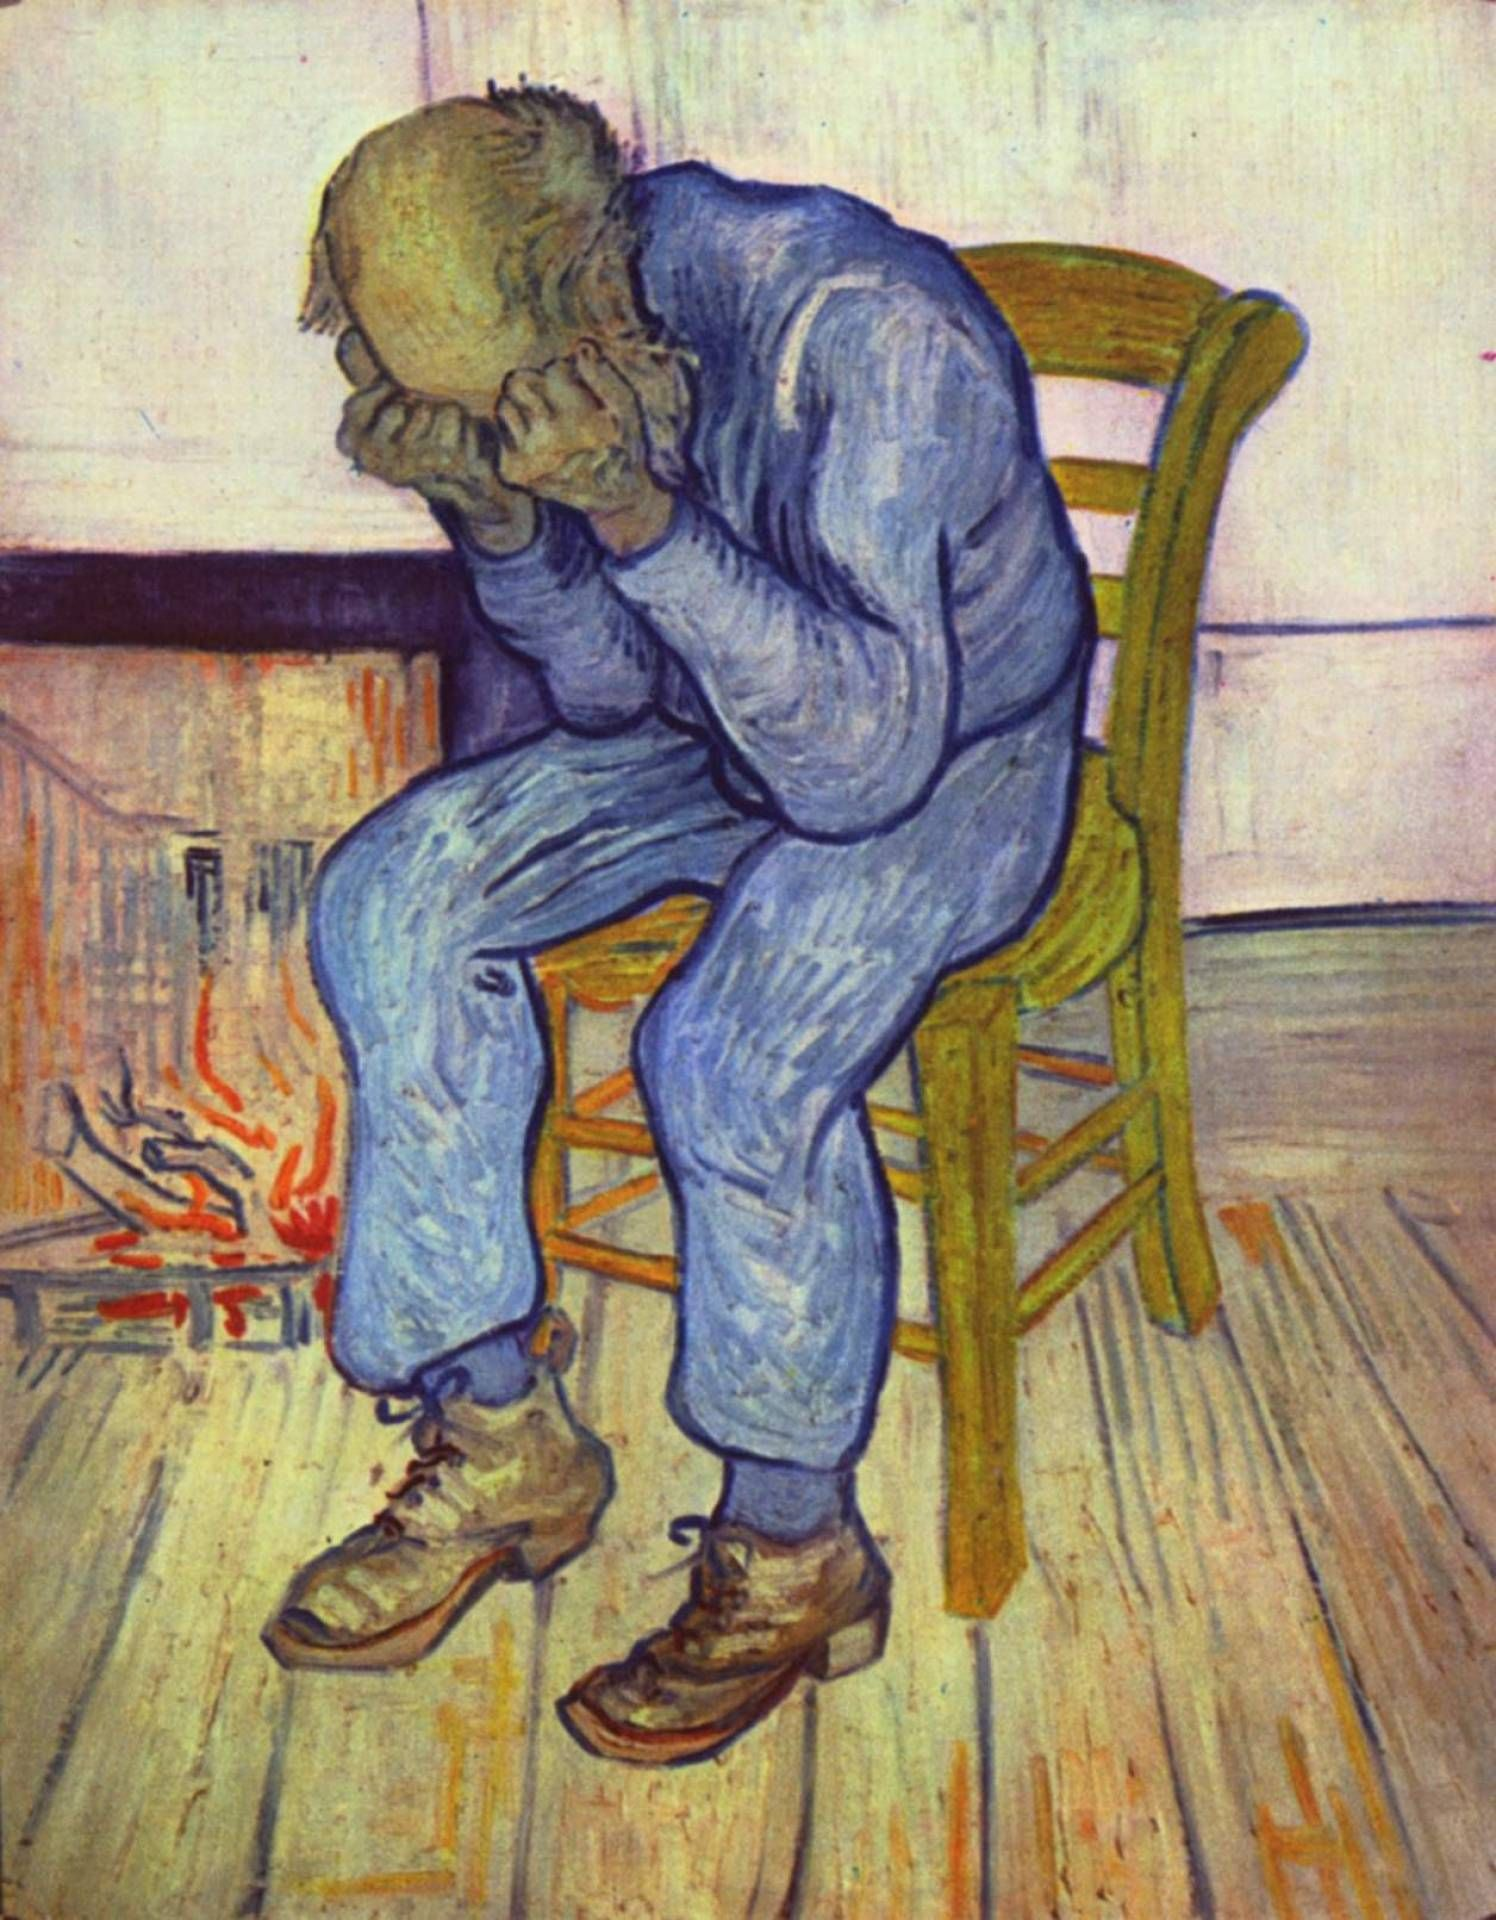
\includegraphics[height=5cm]{./images/dataset/dataset_depression.jpg} \\
    van Gogh's \textit{Depression}
    \end{minipage}
    \begin{minipage}[c]{0.55\textwidth}
    \centering
    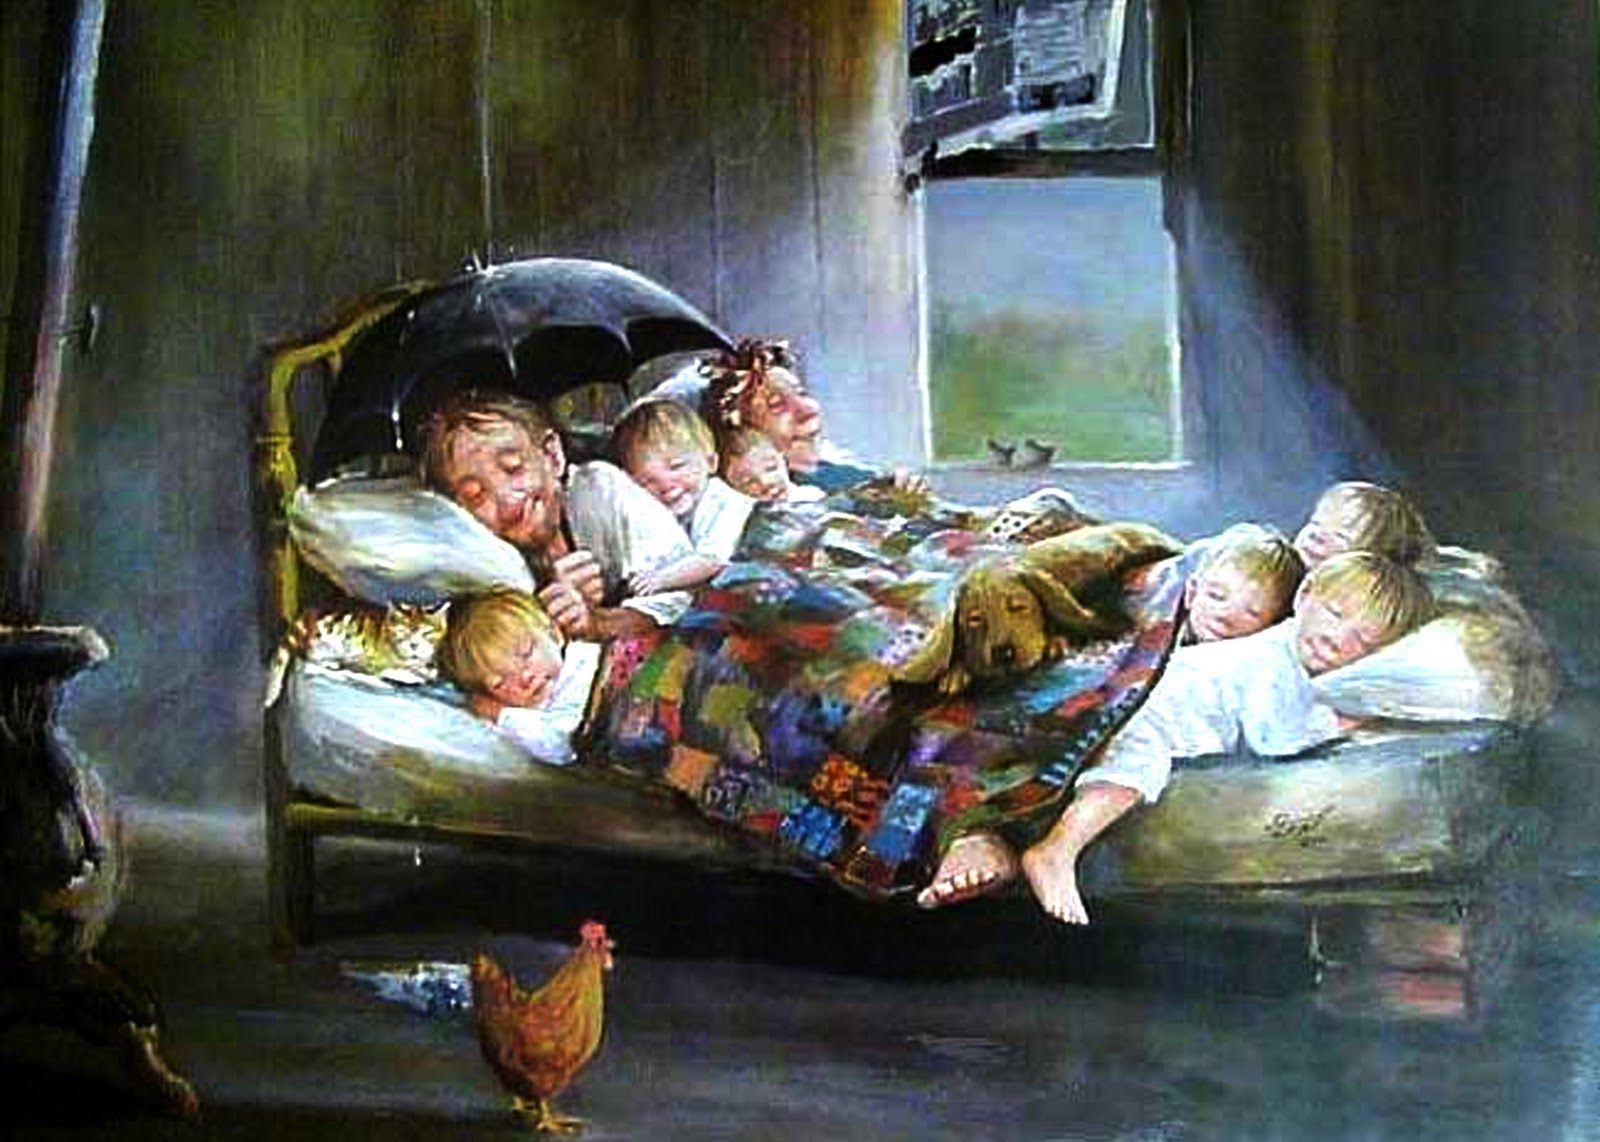
\includegraphics[height=5cm]{./images/dataset/dataset_sweet_home.jpg} \\
    Dengel's \textit{Home Sweet Home}
    \end{minipage}
    \caption{Two emotion eliciting pictures used in the structured interviews.}
    \label{fig:drawing}
\end{figure}

In the corpus, a total of 50 bipolar manic patients (34 male and 16 female) aged between 18 to 54 years are recorded along with 39 healthy controls (23 male and 16 female) aged between 18 to 57 years. Sociodemographics and clinical statistics for two groups are listed in Table \ref{tab:demographic}. 

\begin{table}[ht]
    \small
    \centering
    \caption{Demographic and clinical statistics of BD group and healthy control group}
    \small
    \begin{tabular}{p{1.8cm}|c|c|c|c|c|c}
         \Xhline{2\arrayrulewidth}
         & \multicolumn{3}{c|}{Patients with BD} & & & \\
         & Female & Male & All & Healthy & $t/x^2$ & $p$  \\
         \hline
         Age & $40.2\pm8.8$ & $35.02\pm10.6$ & $36.7\pm10.3$ & $37.3\pm10.9$ & 0.36 & 0.72 \\
         \hline
         Education & $12.6\pm2.9$ & $9.5\pm3.3$ & $10.5\pm3.5$ & $11.2\pm3.7$ & 0.89 & 0.11 \\
         \hline
         Total Episode & $7.13\pm7.7$ & $7.67\pm5.7$ & $6.26\pm6.4$ & - & 0.71 & 0.48 \\
         \hline
         Illness Duration & $15.9\pm9.9$ & $12.02\pm9.7$ & $13.07\pm9.8$ & - & 1.41 & 0.16 \\
         \Xhline{2\arrayrulewidth}
    \end{tabular}
    \label{tab:demographic}
\end{table}


For the classification experiments, the corpus contains 104 recordings as the training partition, 60 recordings as the development partition, and 54 recordings as the test partition, simultaneously balancing the gender distribution. The statistics of recordings refer to Table \ref{tab:recording_length}. The provided ground-truth labels are clinician-annotated YMRS scores of corresponding sessions, and the recordings are also grouped into three disjoint subgroups as follows, thus leading to a ternary classification task.

\begin{itemize}
    \item Remission / Depression: YMRS $\leq$ 7
    \item Hypo-mania: 7 $<$ YMRS $<$ 20
    \item Mania: YMRS $\geq$ 20
\end{itemize}


\section{AVEC2018 Challenge}

Since the automatic recognition of Bipolar Disorder (BD) is recently introduced along with a Turkish-speaking BD corpus, the literature is limited except for the work in the Audio/Visual Emotion Challenge and Workshop (AVEC 2018). AVEC 2018 presented three sub-challenges, and one was BD recognition with Turkish Audio-Visual BD corpus \cite{cciftcci2018}. The organizers \cite{ringeval2018} presented the baseline system for BD recognition, in which only low-level descriptors (LLDs), extracted with open-source toolkits, were used in linear SVM classifiers and the final decision was based on a late fusion of best-performing audio and video representations. In the audio modality, they investigated MFCCs, eGeMAPS, and DeepSpectrum features. DeepSpectrum features were firstly introduced for snore sound classification \cite{amiriparian2017}. Heavily inspired by image processing, DeepSpectrum features were extracted from Mel-spectrogram using the activations from the $2nd$ fully-connected layer of \textit{ALEXNET}. On the other hand, Facial Action Units (FAUs) were used as visual features in the baseline system. The unweighted average recall (UAR) of three symptoms of BD was set as scoring metric, and the best performance on the development partition in the baseline system was 0.635 UAR with the fusion of DeepSpectrum and FAUs.


\begin{table}[htb]
    \centering
    \caption{Comparison of four proposed BD recognition systems in AVEC 2018. The best results are in \textbf{bold} for each metric, and ``dev" and ``test" indicate the performance respectively measured in the development and test set.}
    \begin{tabular}{l|l|l}
        \Xhline{2\arrayrulewidth}
        system & UAR (dev / test) & Accuracy (dev / test) \\
        \hline
        Yang \textit{et al.} 2018 & 0.714 / \textbf{0.574} & \textbf{0.717} / NA \\
        \hline 
        Du \textit{et al.} 2018 & 0.651 / NA & 0.650 / NA \\
        \hline 
        Xing \textit{et al.} 2018 & \textbf{0.868} / \textbf{0.574} & NA / NA \\
        \hline
        Syed \textit{et al.} 2018 & 0.635 / \textbf{0.574} & NA / NA \\
        \Xhline{2\arrayrulewidth}
    \end{tabular}
    \label{tab:four_results}
\end{table}

Against the baseline system, four participating teams presented their BD recognition systems. Yang \textit{et al.} \cite{yang2018} proposed several effective features for the classification: histogram based arousal features, features about speaking rate, and histogram based hands distance features. Along with other histograms of LLDs, these features were reduced in dimensionality and then concatenated before feeding into tree-based classifiers. The histogram-based features enabled the following classification on session-level and the final decision was obtained through a majority vote on an ensemble learning strategy to overcome overfitting issues. The features in visual modality, however, might not capture rapid changes as only histograms emphasized the distribution instead of temporal dependency between features per frame. Moreover, without considering the correlation between modalities, the features lacked robustness as seen in the gap between the performance of development set and test set (shown in Table \ref{tab:four_results}). 

Du \textit{et al.} \cite{du2018} presented a new model called IncepLSTM to encode audio temporal representation on multiple scales with convolutional kernel sizes 1, 3, and 5 in Inception module \cite{szegedy2015}. With an improved triplet loss function to emphasize model sensitivity to the YMRS score, they claimed success to capture dynamic information and to obtain a high-level descriptor for the whole audio clip. Nevertheless, the performance on the development partition is relatively low as seen in Table \ref{tab:four_results} because they only took into account the acoustic modality, resulting in an incomplete utilisation of the available multi-modalities.

Xing \textit{et al.} \cite{xing2018} made full use of all modalities in their framework, including audio, video, and text, which was transcribed with Google Cloud Platform (GCP)\footnote{\url{https://cloud.google.com/translate/}}. They also introduced a hierarchical recall model for the classification, where patients with different mania level were recalled at multiple levels. Each layer within the model contained a Gradient Boosted Decision Tree (GDBTs) using different subsets of all features, and following a boosting strategy, the only un-recalled samples would be transmitted to the next layer. Although the proposed framework yields the highest UAR in the development partition of the four systems, it does not outperform others in the test partition, which indicates their framework might suffer from overfitting due to the noisy data or the limited corpus.

Syed \textit{et al.} \cite{syed2018} proposed ``turbulence features" to capture sudden, erratic changes in feature trajectories, which was measured as the crest factor, the ratio between the absolute maximum value of the signal and its root mean square value, within each window. They applied Fisher Vector (FV) encoding of one modality in feature aggregation and Greedy Ensembles of Weighted Extreme Learning Machines (GEWELMs) in classification. While ``turbulence features" might capture the irregularities in acoustic or visual features, the lack of multi-modal fusion at an early stage leads to the lowest UAR of the four systems as seen in Table \ref{tab:four_results}.




\section{Multimodal Depression Detection Systems}

In addition to the proposed frameworks in AVEC2018, previous research on speech recognition and emotion recognition has demonstrated the effectiveness of some deep architectures on multi-modal data. For audio-visual speech recognition, Ngiam \textit{et al.} \cite{ngiam2011} presented bimodal deep autoencoders to capture the correlations across different modalities and validated the deep architecture on CUAVE and AVLetters datasets. Since it would be difficult to correlate raw data of different modalities, both audio and visual modalities were fused in the shared hidden layer with the learnt first layer representations, which were called ``mid-level" representations \cite{ngiam2011}. Their approach inspired the following work on discovering multimodal features. For emotion recognition, Kim \textit{et al} \cite{kim2013} and Ranganathan \textit{et al.} \cite{ranganathan2016} proposed multi-modal Deep Belief Network (DBN) models, in which ``mid-level" representations on different modalities were connected to one shared hidden layer. With the bimodal representations, they showed an increase in classification performance when compared the baseline system on unimodal features.

Automatic recognition of BD or depression severity, on the other hand, differs from emotion recognition in the processing of temporal information \cite{picard2000, yacoob1994, zacharatos2014}. Dibeklio{\u{g}}lu \textit{et al.} \cite{dibekliouglu2017} presented Stacked Denoising Autoencoders (SDAE) to learn the non-linear mapping of facial landmarks and head pose on frame-level, which was determined by the feature extraction within a specific length of window. An improved Fisher Vector \cite{perronnin2010} was then applied to encode the per-frame representations of visual features into the per-video representations for measurement of depression severity. In their evaluation, dynamics facial landmarks outperformed other modalities and the majority voting \cite{kuncheva2002} of all three modalities showed higher accuracy than unimodal model. 
